%-------------------------------------------------------------------------------
% 请勿删除本注释
% Free Response Question 1
%
% 指引:
% 如在小问之前有通用问题描述,请放置于此
%-------------------------------------------------------------------------------
\begin{figure}[H]
\centering
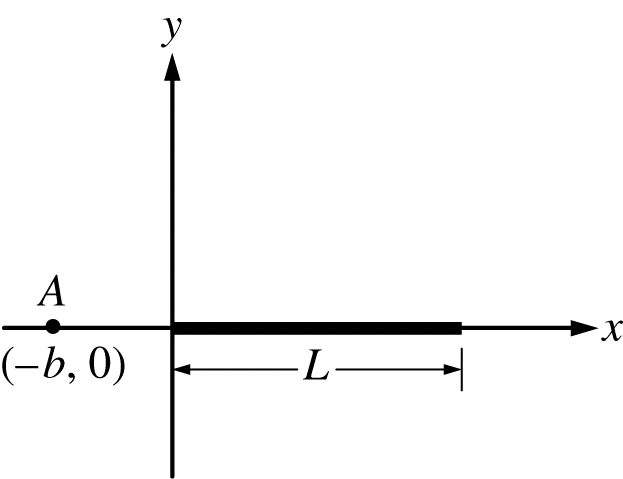
\includegraphics[scale=0.3]{images/img-016-043.png}
\end{figure}


\question
A rod of length $L$ lies along the $x$-axis with its left end at the origin, as shown in the figure above. The rod has a nonuniform linear charge density $\lambda=\alpha x$, where $\alpha$ is a positive constant. % 请删除并替换本行,与上一行 \question 之间不要留空行

\begin{parts}

%-------------------------------------------------------------------------------
% 请勿删除本注释
% Part (a)
%
% 指引:
% 如在小问之前有通用问题描述,请放置于此
%-------------------------------------------------------------------------------

\part
Determine the units of the constant $\alpha$. % 请删除并替换本行,与上一行 \part 之间不要留空行

%-------------------------------------------------------------------------------
% 请勿删除本注释
% Part (b)
%
% 指引:
% 如在小问之前有通用问题描述,请放置于此
%-------------------------------------------------------------------------------

\part
Derive an expression for the total charge on the rod. Express your answer in terms of $\alpha, L$, and physical constants, as appropriate. % 请删除并替换本行,与上一行 \part 之间不要留空行

%-------------------------------------------------------------------------------
% 请勿删除本注释
% Part (c)
%
% 指引:
% 如在小问之前有通用问题描述,请放置于此
%-------------------------------------------------------------------------------

The rod is replaced with one of the same length but with a uniform positive linear charge density $\lambda_{0}$.

\part
Show that the electric field at point $A$, which is a distance $b$ to the left of the rod, has a magnitude of
$E=\frac{\lambda_{0} L}{4 \pi \varepsilon_{0} b(b+L)}.$
 % 请删除并替换本行,与上一行 \part 之间不要留空行

%-------------------------------------------------------------------------------
% 请勿删除本注释
% Part (d)
%
% 指引:
% 如在小问之前有通用问题描述,请放置于此
%-------------------------------------------------------------------------------

\part
A proton is placed at point $A$, at position $(-b, 0)$, near the positively charged rod and released from rest. % 请删除并替换本行,与上一行 \part 之间不要留空行
\begin{subparts}
\subpart Sketch a graph of the horizontal component of the acceleration of the proton $a_{x}$ as a function of its position $x$ for the region in which the proton travels after it is released. Sketch any asymptote, but do not indicate its value.

\begin{figure}[H]
\centering
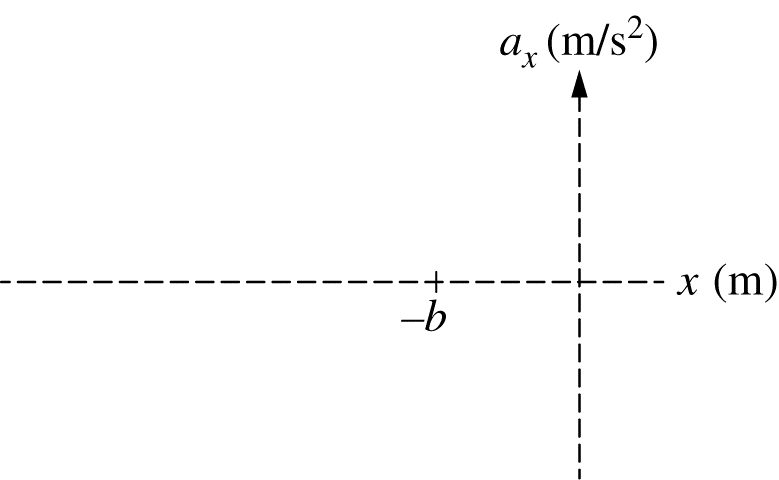
\includegraphics[scale=0.3]{images/img-017-044.png}
\end{figure}

\subpart Sketch a graph of the horizontal component of the velocity of the proton $v_{x}$ as a function of its position $x$ for the region in which the proton travels after it is released. Sketch any asymptote but do not indicate its value.

\begin{figure}[H]
\centering
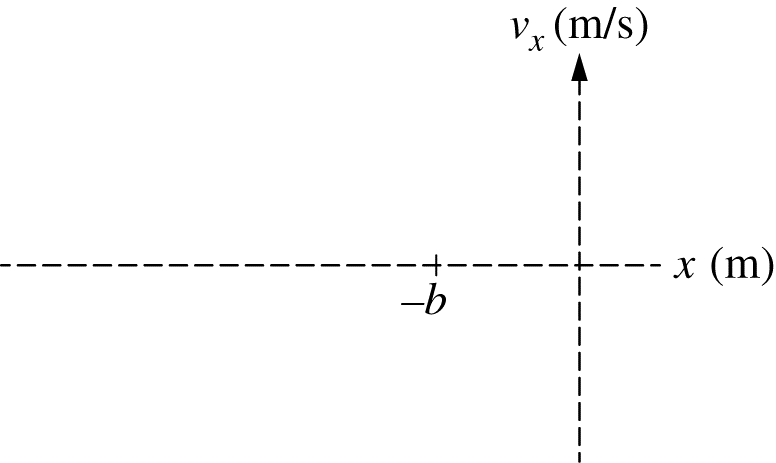
\includegraphics[scale=0.3]{images/img-017-045.png}
\end{figure}

\subpart Instead of a proton, an alpha particle (a particle with twice the charge and four times the mass of a proton) is now placed at point $A$. Is the magnitude of the initial acceleration of the alpha particle greater than, less than, or equal to the magnitude of the initial acceleration of the proton from part $(d) i ?$
\end{subparts}

\underline{\qquad}Greater than \qquad  \underline{\qquad}Less than \qquad  \underline{\qquad}Equal to

%-------------------------------------------------------------------------------
% 请勿删除本注释
% Part (e)
%
% 指引:
% 如在小问之前有通用问题描述,请放置于此
%-------------------------------------------------------------------------------

\part
Using the equation from part (c), show that the magnitude of the electric field at a point on the $x$-axis very far away from the rod is approximately equal to the electric field due to a point charge of magnitude $Q=\lambda_{0} L$ located at the origin. % 请删除并替换本行,与上一行 \part 之间不要留空行

\end{parts}
